% Cover letter using letter.cls
\documentclass[a4paper]{scrreprt} 
%\usepackage{helvetica} % uses helvetica postscript font (download helvetica.sty)
%\usepackage{newcent}   % uses new century schoolbook postscript font 
\usepackage[utf8]{inputenc}
\usepackage{graphicx}
\usepackage{amsmath}
\usepackage{eurosym}
\usepackage{cite}
\usepackage{tabularx}
\usepackage{bytefield}
\usepackage{color}
\usepackage{longtable}
\usepackage{tabularx}
\usepackage[bookmarks]{hyperref}
\hypersetup{pdftex,colorlinks=true,allcolors=black}
\usepackage{hypcap}
% the following commands control the margins:
%\topmargin=-1in    % Make letterhead start about 1 inch from top of page 
%\textheight=8.5in    % text height can be bigger for a longer letter
%\oddsidemargin=0pt   % leftmargin is 1 inch
%\textwidth=6.5in     % textwidth of 6.5in leaves 1 inch for right margin
\title{Implementing a temperature and humidity sensor network for the nEDM
experiment setup}
\author{Wenwen Chen, Rainer Schönberger}
\begin{document}
\maketitle
\tableofcontents
\input{Concept}
\section{Features}
\section{Sensors}
\subsection{TSIC 506F}
For temperature measurements, we use the TSIC 506F temperature sensor
integrated circuit. At a relatively low price of about \EUR{7} per device, it
is able to deliver very high accuracy (see table \ref{tab:tsic}).\\
The temperature is converted to a digital value, which is sent out over a
proprietary one wire protocol variant, called \emph{ZAC-Wire}. The Transmission structure can be seen in figure \ref{fig:tsic_transmission}. Details about the ZACwire protocol are described in section \ref{chap:zac}.\\
The temperature $T_{cels}$ in celsius can be calculated from the received value $T_{dig}$ using
$$T_{cels} = \frac{T_{dig}}{2047} \cdot 70\,^{\circ} - 10\,^{\circ}.$$
In order to minimize soldering heat, which would influence the calibration, we used the TO92 packaged sensor.
\begin{table}[Hh!]
	\centering
	\begin{tabular}{| r | c |}
		\hline
		Temperature range & $-10\,^{\circ}\mathrm{C}$ to $60\,^{\circ}\mathrm{C}$\\
		\hline
		Calibrated accuracy & $\pm 0.1\,\mathrm{K}$  \\
		\hline
		Resolution & $0.034\,\mathrm{K}$  \\
		\hline
	\end{tabular}
	\caption{TSIC 506F specs}
	\label{tab:tsic}
\end{table}
\begin{figure}[Hh!]
	\centering
	\definecolor{lightgray}{gray}{0.8}
	\begin{bytefield}[endianness=big, bitwidth=2.1em]{10}
		\bitheader{0-9}\\
    \bitbox{1}{ST} & \bitbox{5}{0} & \bitbox{3}{$T_{dig}$[10:8]} & \bitbox{1}{P}\\
    \bitbox{1}{ST} & \bitbox{8}{$T_{dig}$[7:0]} & \bitbox{1}{P}
	\end{bytefield}
  \caption{TSIC transmission structure. The temperature is sent over the wire, with two ZACwire transmissions. P is an even parity bit. ST is the start bit.}
	\label{fig:tsic_transmission}
\end{figure}
\subsection{HYT271}
\section{Logical design}
Our network architecture is structured into 3 parts (see figure \ref{fig:topo}):
\begin{description}
  \item[Measuring:]
    Sensors do periodic measurements. The results are transmitted,
    using an unified protocol. We used ZACwire, as the unified
    protocol, as in our application we have more temperature sensors
    than humidity sensors, which natively speak ZACwire. Hence no
    protocol conversion will be required for the majority of the
    sensor boards. To extend the range and noise behavior, we use
    RS485 as a physical layer protocol, to transport the ZACwire
    signal.
  \item[Data acquisition:]
    At this part of the network, the ZACwire signal from the sensors
    is interpreted and buffered. The measurement data is then
    provided over an I2C interface.\\
    In our implementation, we support receiving of up to 8 Sensors
    per collector board. To increase the numbers of sensors in the
    network, multiple collector boards may be connected to the I2C
    bus, using the I2C chaining connectors. Using this technique,
    the network theoretically may consist of up to
    $128\cdot 8 = 1024$ sensors.
  \item[Data forwarding:]
    The forwarding part controls the data aquisition part of the
    network and provides an interface to IP networks. Data may be
    forwarded to a couchDB database on the internet and the network
    can be configured via an telnet terminal user interface.
\end{description}
\begin{figure}
	\centering
	
\includegraphics[width=0.9\textwidth]{img/plan2.pdf}
	\caption{Network topology}
	\label{fig:topo}
\end{figure}
\section{Protocols}
\subsection{ZACwire}\label{chap:zac}
ZACwire is a prorietary one wire comminucation protocol, developed
by IST AG. Only one data line is needed.\\
Bits are represented by
different duty cycles of the waveform within the bit time $T_b$.
Every normal bit starts and ends with a falling edge. At the beginning
of each transmission, a start bit with a duty cycle of 50\% is
transmitted. From this start bit, the bit time $T_b$ for the
transmission can be extracted. If the bus is high for a time $>T_b$
the transmission ends, this is called a Stop bit. Figure \ref{fig:zac}
shows the four different wafeform types, of which a ZACwire signal may be
composed off. Figure \ref{fig:zacexample} shows an example
transmission.
\begin{figure}[b]
	\centering
	
\includegraphics[width=0.3\textwidth]{img/zac_bits.pdf}
	\caption{ZACwire protocol signal interpretation}
	\label{fig:zac}
\end{figure}
\begin{figure}[b]
	\centering
	
\includegraphics[width=0.9\textwidth]{img/zac_example.pdf}
	\caption{ZACwire protocol example}
	\label{fig:zacexample}
\end{figure}
\subsection{I2C}
I2C is a bus protocol, which specifies the physical layer, as well as an arbitration and addressing layer. The protocol allows communication between multiple bus participants.\\
Transmissions are done over two transmission lines SCL and SDA, which
are pulled to logical high voltage level by pullup resistors (see
figure \ref{fig:i2c}). Each transmission is controlled by a device
in master mode, which provides a clock by controlling the SCL line.\\
A transmission is surrounded by a START and a STOP bit, which are code violations.\\
At the beginning of a transmission, the master first transmits an
address to the bus, addressing one or all connected devices which
are in slave mode. After that a data direction bit is sent to the
bus, which defines the slave behavior. If the direction bit specifies a write, all addressed slave devices read bits from the bus at every 
lock cycle, the SDA line stats under control of the master. If the
direction bit describes a read, the slave should take control over
the SDA line and transmits bits at every clock cycle.\\
The Slave is allowed to take control over the SCL line at any time
by pulling it low. this is called clock extenstion, and signals the
master to not proceed transmitting or receiving data.
\begin{figure}
	\centering
	\includegraphics[width=0.7\textwidth]{img/i2c.pdf}
  \caption{I2C logical bus structure. Source \ref{}.}
	\label{fig:i2c}
\end{figure}

\subsection{RS485}
RS485 is a transmission line standard, which specifies differential line communication over twisted pair cables. It allows very long distance communication of up to 1 kilometer with high noise immunity and reduced noise emission.\\
Figure \ref{fig:rs485} illustrates the working principle of the protocol. The encoder transforms a single bit line DI into two separate lines A and B. If DI is high, the output voltage at line A, $V_{OA}$ will bigger than at line B ($V_{OB}$). If the input voltage at DI is low, $V_{OB}>V_{OA}$ holds.\\
\begin{figure}[b]
	\centering
	\includegraphics[width=0.7\textwidth]{img/rs485.pdf}
  \caption{RS485 encoding/decoding - Logical structure. Source: \ref{XXX}.}
	\label{fig:rs485}
\end{figure}

\chapter{Implementation}
\section{Toolchain}
\subsection{ISP programming}
To upload the compiled code and to configure the microprocessors, we used the USBasp programmer in combination with the avrdude software.\\
As we needed to access the fuse bytes of the arduino too, which was not possible with the arduino bootloader, we also use the ISP header on the Arduino board for programming. The arduino bootloader was removed. Hence it is not possible anymore, to programm the arduino with the arduino software suite, without reinstalling the bootloader.\\
Note that the arduino ISP header is not compatible with the one, provided by the USBasp programmer. A mechanical adaptor or individual cabling is required. Figure \ref{XXX} shows the pin asignments of the different ISP headers.
\subsection{USART for debugging}
For convenient debuging, we added a USART header on each board with a microcontroller. These pins are directly connected to the hardware USART unit of the
microconteoller. Note, that the signal level on this header is TTL and is not compatible with the RS232 standard. Using either an external signal level converter from TTL to RS232, or a direct USB to USART TTL converter, it is possible to connect the boards to a PC.\\
In every software component, we set the \emph{stdout} file descriptor, to point to a USART file, implementing writing data to the USART line.
Hence standard file handling functions like \emph{printf} or \emph{puts} can be used.\\
To read and write data at the PC side, software like \emph{screen} or \emph{picocom} may be used. The default baudrate is 9600bps.
\subsection{Build process}
To build and upload the code the following software and libraries are required:\\
Tools:
\begin{itemize}
  \item avr-gcc
  \item avr-objcopy
  \item avrdude or other ISP programming software
\end{itemize}
Libraries:
\begin{itemize}
  \item avr-libc
  \item Arduino ethernet library (only for ethernet board)
  \item Arduino core library (only for ethernet board)
\end{itemize}
We use the make build environment. The Makefiles in each software directory contain instructions on how to build and upload the software to the microcontroller, using the following rules:
\begin{description}
  \item[make clean] Clears the build directory.
  \item[make] Compiles and links the source code to the elf and intel hex binary format. Also a eeprom image is generated in intel hex binary format. The output directory for binary files will be \emph{./build/}.
  \item[make fuse] Configures the controller, to use the right system clock source, burnout detection and eeprom persistency settings.
  \item[make eeprom] Uploads the eeprom image to the controller.
  \item[make upload] Uploads the compiled software to the microcontroller, using avrdude. By default the usbasp programmer is selected.
\end{description}
For a first time build and upload, the above order should be respected. After the initial upload, fuses and eeprom should not be touched everytime, the software changes.\\
To be able to find the Arduino library root path, the \emph{ARDUINO\_PATH} environment variable should be set to the Arduino installation directory. This for example is the Path to the cloned Arduino git reporitory.\\
Note, that the Makefiles in the current version, do not automatically search for file dependancies, hence a make clean should be executed, after every change in not explicitly specified files, namely every non .c or .cpp file.
\section{Temperature board} \label{chap:tempbrd}
The temperature board consists of the TSic506F sensor and
complementary circuitry. The ZACwire signal is transformed to the
RS485 electrical layer, using a ST485 integrated circuit. The board
provides a RJ45 socket,  over which the required supply voltage of 5V
should be provided, and the two differential signal outputs can be
received. The schematic diagram can be seen in figure
\ref{fig:schem_temp}.\\
Care was taken, when soldering the temperature sensor, to minimize
heat transfer to the chip. We did this by soldering each pin for a
maximum time of 2 seconds, We also tried to keep the total time spent
for soldering all 3 pins less than 10 seconds. After soldering, we
immediately blowed cold air to the pins and the chip itself.
\begin{figure}
	\centering
	\includegraphics[width=0.6\textwidth]{img/schem_temperature_board.pdf}
	\caption{Temperature board schematic. The Impedance adjustor circuit, R4 and C4 is not required to be populated, as we only transmit data.}
	\label{fig:schem_temp}
\end{figure}
\section{Humidity board}
\subsection{Hardware}
The hardware structure is similar to the temperature board, described in section \ref{chap:tempbrd}. However, as the HYT271 sensors use I2C for
communication, we added a microcontroller to repediately poll the sensor for current measurement results and send the data out, using a software
implementation of the ZAC wire protocol. Therefore we also placed an ISP socket, a debugging adapter, a reset switch and two LEDs onto the board, which makes it
slightly bigger than the temperature board. The schematic can be seen in figure \ref{fig:schem_hum}.
\begin{figure}
	\centering
	\includegraphics[width=0.8\textwidth]{img/schem_humidity_board.pdf}
	\caption{Humidity board schematic}
	\label{fig:schem_hum}
\end{figure}
\subsection{Software}
\section{Collector board}
The collector board decodes the ZAC protocol and provides an I2C interface for
reading out temperature, as well as humidity values of connected sensors.
Care was taken, to ensure a response time of $<1\,\mathrm{s}$.
\subsection{Hardware}
The schematic diagram can be seen in figure \ref{fig:schem_collect}. The hardware consists of the following main components:
\begin{description}
  \item[Microprocessor:]\hspace{1cm}\\
    To do all protocol conversion tasks, we used an Atmel Atmega88PA
    microcontroller, running at a clock speed of $20MHz$. The clock
    is generated, using an external crystal oscillator.\\
    The Atmega microconteoller provides a variety of useful features
    like asynchronous timers, pin change interrupts on every GPIO
    pin, hardware support for the I2C protocol and integrated EEPROM
    storage.\\
    We connected the sensors in two groups, so that we are able to
    receive two independent interrupts for two sensors in different
    groups.
  \item[I2C connection:]\hspace{1cm}\\
    The board provides two 6 pin IDC pin headers (P3 and P4), which
    provide connection to the I2C bus, as well as an optional 5V
    power line (Vi2c). The two headers are connected in parallel,
    so they can be used for chaining multiple collector boards.\\
    The board also has integrated I2C pullups, which can be enabled
    using the switch SW2, in case the I2C master does not provide
    pullups.
  \item[Sensor connection:]\hspace{1cm}\\
    The individual sensors are connected via an eight-port RJ45
    socket header. The signal of each sensor is first interpreted
    by an RS485 transceiver and afterwards directly provided to a
    microcontroler GPIO pin. As this is the receiving side, we also
    had do add impedance matching circuitry. We chose to implement
    a power saving AC-termination solution, as suggested in \ref{XXX}.
    To bring the output level of each transceiver to a defined state,
    when no sensor is connected, we use pullup resistors on the
    input side.
  \item[Developer interface:]\hspace{1cm}\\
    The microcontroller can be programmed with any AVR In System
    Programmer, using the standard ISP header (P8).\\
    For debugging code, we also added a USART pin header (P1), which
    allows serial communication with the microcontroller. Care
    has to be taken, when connecting the chip to a PC, as the logic
    levels of our board are 5V TLL and hence are not compatible
    with the RS-232 logic levels, used by most PCs. We suggest to use
    a USB to USART TLL converter or a logic level converter.
  \item[Power source:]\hspace{1cm}\\
    We provide multiple ways to supply power to the collector board.
    \begin{itemize}
      \item Direct 5V input/output (P7 or P9)
      \item Use the 5V supply voltage, provided via the I2C bus
      \item Unregulated input (7V..25V). The onboard LM7805 linear
        regulator, will convert the voltage to 5V.
    \end{itemize}
    Using the pin header K1, it is possible to select suitable
    power inputs.\\
    Example 1: If the board should get power over I2C, pins 1 and 2
    should be shorted.\\
    Example 2: If the board should get power from the on board
    regulator, and also provide power to the I2C bus, all three pins
    should be shorted.
\end{description}
\begin{figure}
	\centering
	\includegraphics[width=1\textwidth]{img/schem_collector_board.pdf}
	\caption{Collector board schematic}
	\label{fig:schem_collect}
\end{figure}
\subsection{ZAC decoding}
AVR controllers do not have hardware support for decoding the ZAC one wire
protocol (protocol definition is explained in chapter \ref{chap:zac}). Hence we
implemented a software decoder. However our implementation
does not follow the method suggested by \cite{zac} because of timing reasons.\\
To decode one ZAC protocol sensor, we use one 8 bit timer, the corresponding timer
overflow interrupt and the pin change interrupt (PCINT) of the pin, connected to the sensor.
\paragraph{Pin change Interrupt:} On every pin change interrupt, the following actions are executed:\\
Every time:
\begin{itemize}
	\item The current current value is stored to a temporary variable $T_{timer}$, to be able to still access it later.
	\item The timer is reset.
	\item If the timer is not jet running, it is started now.
\end{itemize}
On a falling edge:
\begin{itemize}
	\item If $\left|T_{low} - T_{timer}\right| < T_{thresh}$ with a constant $T_{thresh} << T_{crit}$, we
		have observed a start bit.\\
		We now update the critical sampling time\footnote{$T_{crit} = 0.5\cdot(T_{timer} + T_{low})$ would
		be more accurate, but would consume more time to calculate.}: $T_{crit} = T_{timer}$.
\end{itemize}
On a rising edge:
\begin{itemize}
	\item The current timer value is stored as $T_{low}$. If we already observed a falling edge, this
		represents the time, the signal was low.
	\item If we already have seen a start bit, we now sample a data bit\footnote{Note, that a repeated
		start bit would also be sampled as a data bit with an unpredictable value.}:\\
	$\mathrm{bit} = \begin{cases} 1 & \text{if } T_{timer}<T_{crit} \\ 0 & \text{else}\end{cases}$
\end{itemize}
\paragraph{Timer overflow Interrupt:} The timer is configured in a way, that an overflow will occur after
the timer is running without a reset for $T_{ovf}$, with $T_{bit} < T_{ovf} < 100\,\mathrm{ms}$. Hence
the interrupt will occur, after a completed transmission and before the start of the next transmission.\\
After a overflow occurs, we check, if we received a whole transmission. If this is the case, we disable
interrupts and stop the current measurement. Otherwise we reset the receive buffer and wait for the
next transmission to begin.
\paragraph{Starting a measurement:} To start the meassuring process, the following is executed:
\begin{itemize}
	\item $T_{crit}$ is set to the maximum value.
	\item $T_{low}$ is set to the minimum value. This will ensure, that we do not
		accidentally recognize the first falling edge as a start bit.
	\item The receive buffer is reset.
	\item Interrupts are enabled.
\end{itemize}
%\paragraph{}
Our algorithm is not able to see stop bits correctly, if $T_{ovf}$ is configured badly.
However in our case we deliberately configured $T_{ovf}$ to be bigger that the maximum
high time in case of a stop bit.
This allows us to only see the end of the complete transmission, as a TSIC sensor also
sends a useless stop bit after the first 9 bits.\\
%\paragraph{}
As we have up to 8 sensors connected to the Atmega88, we have to do one measurement
after another. as one sample of a measurement takes $>100\,\mathrm{ms}$ we would run
into problems reaching the desired sampling rate of $>1\,\mathrm{Hz}$.
Our approach is to sample two sensors at the
same time, using a second 8 bit timer. Our interrupt handler for the ZAC protocol decoding are not interruptable.
Hence, incomming interrupts are delayed for the runtime $t_e$ of currently executed interrupts.
If we have interrupts active for two sensors at the same time, the controller might see a delayed signal.
\begin{figure}[b]
	\centering
	\includegraphics[width=0.7\textwidth]{img/zac_timing.pdf}
	\caption{ZAC protocol worst case timing. The grey shaded areas illustrate the potentially delayed vision
	of a microcontroller due to interrupt latency.}
	\label{fig:zactiming}
\end{figure}
Figure \ref{fig:zactiming} illustrates this problem:\\
When sampling the start bit we get an error for our critical time $T_{crit}$:
$$T_{min} := T_h - t_e < T_{crit} < T_h + t_e$$
When using $T_{crit}$ to determine a bit value, we are again influenced by the possibly delayed preceeding falling edge. We get:
$$T_{min} < T_{crit}' < T_h + 2 \cdot t_e =: T_{max}$$
Our algorithm will only work correctly, if
$$T_{min} > 0.5\cdot T_h + t_e$$
or
$$T_{max} < \frac{3}{2}\cdot T_h\text{.}$$
Both inequations simplify to
$$t_e < \frac{1}{4}\cdot T_h\text{.}$$
According to \cite{zac}, the nominal value for $T_h$ is $\frac{125}{2}\,\mu\mathrm{s}$. Hence our error due to
interrupt latency has to be smaller than $15.625\,\mu\mathrm{s}$.\\
As the microcontroller runs at a clock speed of $20\,\mathrm{MHz}$, we have to complete previous interrupts,
start the interrupt handler of the new interrupt and sample the current timer value within 332 clock cycles,
to not harm the above limit on the error.\\
We implemented a simple branch aware Worst Case Execution Time (WCET) analyzer for the AVR instruction set.
It is able to calculate the maximum execution time of individual sections in the compiled code\footnote{Note that,
whereas branches are considered, only branches to addresses in the future are handled correctly. Loops i.e.
branches to already executed code cause undefined, possibly non terminating behaviour of the analyzer. As our code
does not contain loops, this did not cause problems and loop handling was not implemented.}. Figure \ref{fig:wcet}
shows the WCET analyzer output for the Pin change interrupt handler. The worst case execution time for the total
handler is $100$ cycles. The timer interrupt takes less than $50$ cycles to complete. For a complete analysis one
additionally has to consider the time for jumping to the interrupt handler ($<20$ cycles) and the time we need to read out the
timer value in the new interrupt handler ($<29$ cycles). This gives us a total latency of less than $199$ clock
cycles, which is well within the allowed range.
\begin{figure}
	\centering
	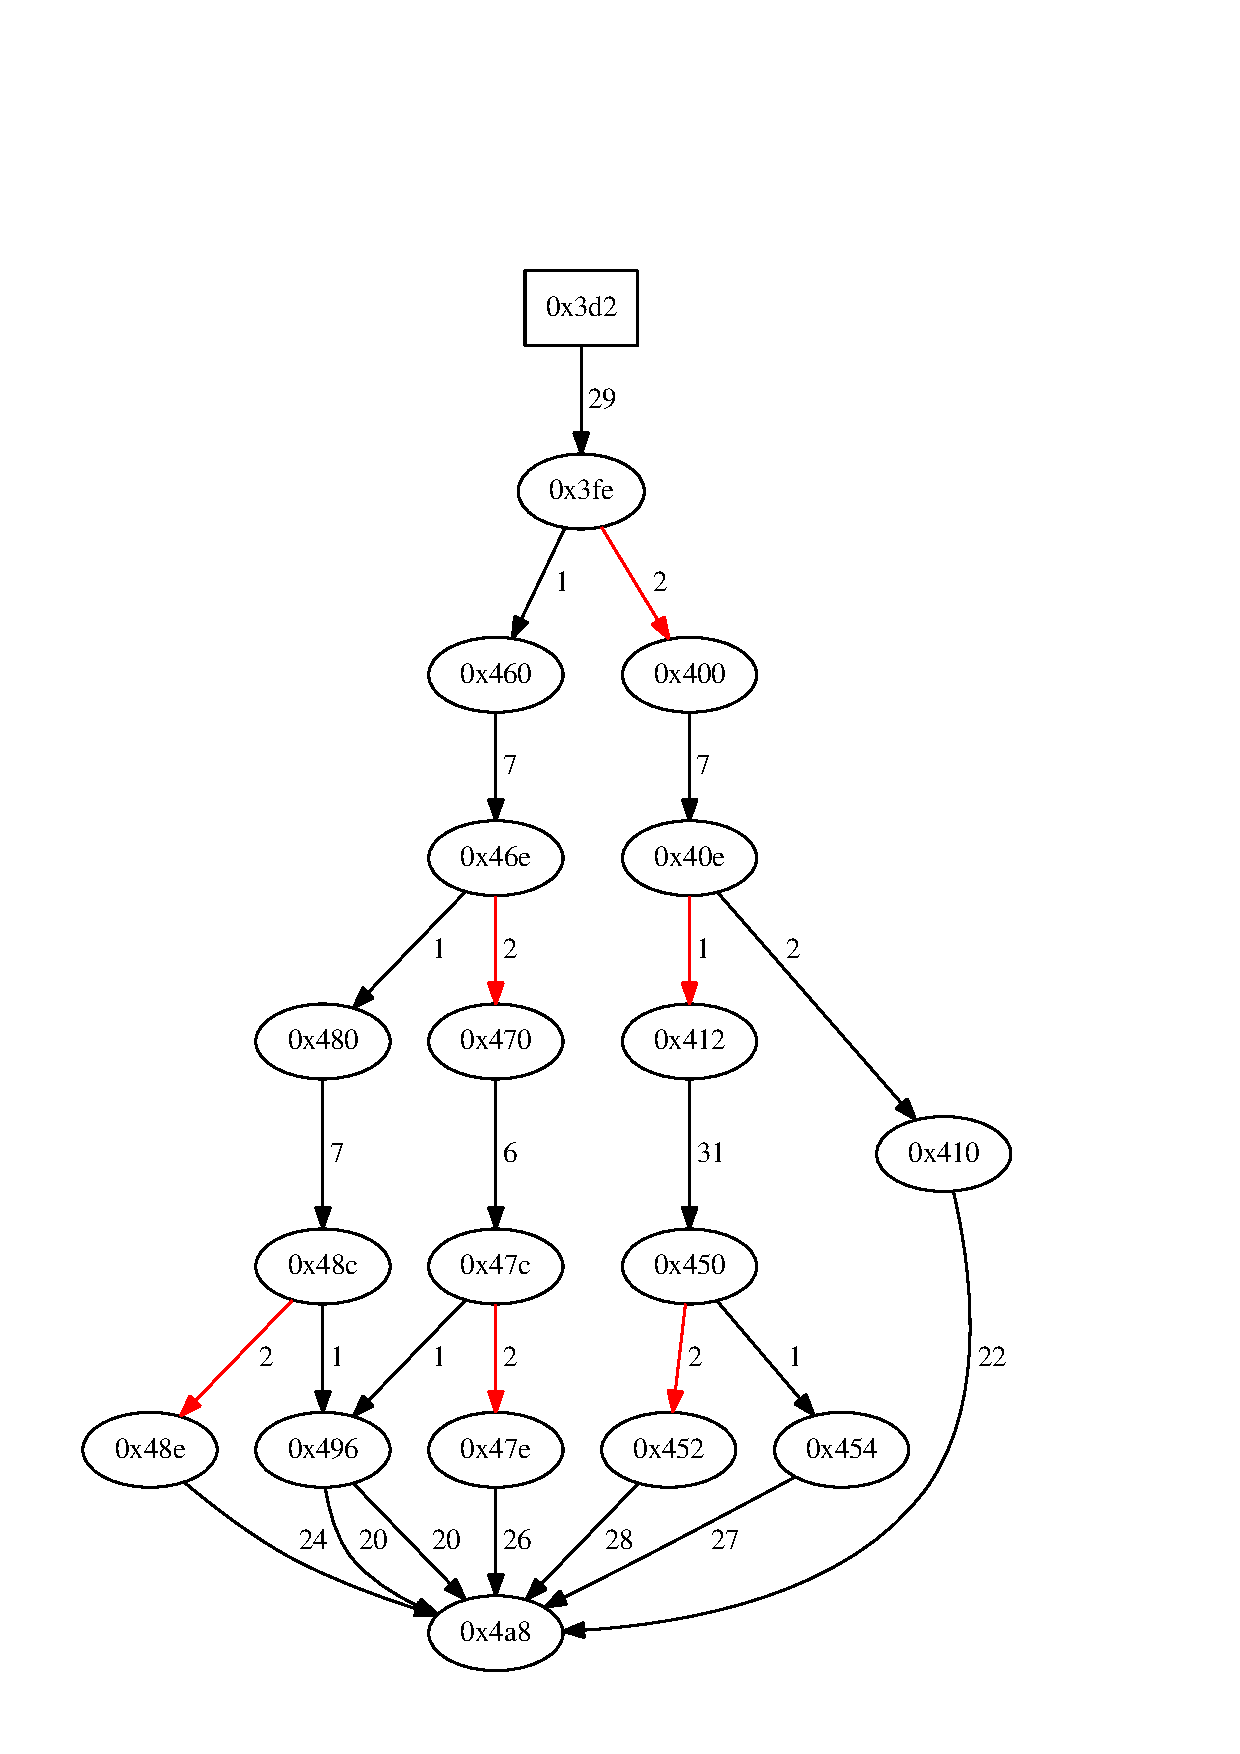
\includegraphics[width=0.5\textwidth]{img/wcet/vector_4.pdf}
  \caption{Branch aware WCET analysis of the Interrupt handler for vector\_4 (Pin change interrupt).
  Nodes represent program addresses, arrows represent branches. Red arrows point to the branch with the
highest execution time. The values near the arrows represent the execution time from the previous node's
address to the instruction causing the branch.}
	\label{fig:wcet}
\end{figure}
\subsection{I2C interface}
Communication with the collector board is done via I2C (Two Wire Interface). Thereby the board acts as an
I2C slave, extending the clock, if it is currently not able to process incomming data.
This is especially used while a measurement is in progress: As soon as new data byte arrives,
it is buffered and the clock will be extended, signalling to the master, that no further data should be sent or received.\\
If a write request (SLA+W) is sent, the following data is interpreted as a command. A list of implemented commands is given
in table \ref{tab:i2c}. The collector board reacts to the general call address 0. This makes it possible to trigger a measurement
on multiple boards, using only one I2C transmission. Also the own I2C address can be set to a new value without knowing the old one.\\
If a read request (SLA+R) is sent, the packet array from the last completed measurement will be sent out, starting with sensor 0.
For details about the packet format see chapter \ref{chap:packet}. Not all packets have to be received, as soon as a STOP bit is
received, the transmission is aborted. A new read request will again trigger the transmission of data starting at sensor 0.
\begin{table}[Hh!]
	\centering
	\begin{tabularx}{\textwidth}{ | c | c | c | X | }
		\hline
    Name & Value & Parameters & Action\\
		\hline
		\hline
    START\_MEASUREMENT & 0x01 & --- & All 8 sensor values will be
    captured as soon as the STOP bit is received. If during
    measurement
		the slave is addressed again, the I2C clock will immediately be extended until the measurement is complete, blocking the whole I2C bus.\\
		\hline
    SET\_ADDRESS & 0x02 & address & The own I2C address will be updated with the 1 byte value following the command. The address should
		be in the range from 8 to 112. The default address is 42\\
		\hline
    LED\_ON & 0x03 & number & The LED with the given number will be turned on.\\
		\hline
    LED\_OFF & 0x04 & number & The LED with the given number will be turned off.\\
		\hline
	\end{tabularx}
	\caption{List of implemented I2C commands}
	\label{tab:i2c}
\end{table}
\subsection{Measurement packet format}\label{chap:packet}
After data was received via the ZAC-Wire protocol, it is interpreted and converted to a convenient packet format, suitable for
redirection via I2C. Each packet's integrity is protected by a CRC checksum and consists of the following fields:\\
\begin{description}
	\item[\textbf{type}] This field pecifies the type of the sensor, which supplied the data. Currently implemented values are 0
		for TSIC and 1 for HYT. In case the type field reads 0, the \emph{Humidity} field will have no relevant value hence
		represents a padding field.
	\item[c] This bit is set to 1, if the measurement was completed without a timeout. This is usually the case, when a
		sensor is connected. Hence this bit can be used to determine, whether a sensor is connected or not.
	\item[error] This field reads 1, when an error during sampling has occured. Possible causes are: HYT Checksum missmatch,
		TSIC Parity missmatch or TSIC Protocol format error.
	\item[Temperature] $T_m \cdot 100$ with $T_m$ the measured temperature in Celsius.
	\item[Humidity] $RH_m \cdot 100$ with $RH_m$ the measured relative humidity in \%.
	\item[CRC-8] Checksum over the first 5 bytes of the packet\footnote{The Humidity field is always part of the checksum
		calculation, even if the packet type is 0.}.
\end{description}
Figure \ref{fig:packet} shows the structure of a packet. Packets can be received via I2C in the order, shown in
figure \ref{fig:packetorder}.\\

\begin{figure}
	\centering
	\definecolor{lightgray}{gray}{0.8}
	\begin{bytefield}[endianness=big, bitwidth=2.1em]{8}
		\bitheader{0-7}\\
		\begin{rightwordgroup}{Header}
			\bitbox{2}{type} & \bitbox{3}{\color{lightgray}\rule{\width}{\height}} & \bitbox{1}{c} & \bitbox{2}{error}
		\end{rightwordgroup}\\
		\begin{rightwordgroup}{Payload}
			\wordbox{2}{Temperature}\\
			\wordbox{2}{Humidity}
		\end{rightwordgroup}\\
		\wordbox{1}{CRC-8}
	\end{bytefield}
  \caption{Packet format of a measurement. The whole packet is 6 bytes long}
	\label{fig:packet}
\end{figure}
\begin{figure}
	\centering
	\definecolor{lightgray}{gray}{0.8}
	\begin{bytefield}[endianness=little, bitwidth=0.7em]{48}
		\bitheader{0,6,12,18,24,30,36,42}\\
		\bitbox{6}{Sensor 0} &
		\bitbox{6}{Sensor 1} &
		\bitbox{6}{Sensor 2} &
		\bitbox{6}{Sensor 3} &
		\bitbox{6}{Sensor 4} &
		\bitbox{6}{Sensor 5} &
		\bitbox{6}{Sensor 6} &
		\bitbox{6}{Sensor 7}
	\end{bytefield}
  \caption{Transmission packet order}
	\label{fig:packetorder}
\end{figure}

\section{Ethernet board}
\subsection{Hardware}
\subsection{Software}
\subsection{User interface}
The ethernet board provides a terminal user interface over TCP/IP, which may be accessed via applications like telnet or netcat.
This allows users to conveniently change or view system settings. The interface is command driven, every command should be terminated
by a newline and/or carrier return character.\\
By default, the user interface is reachable at port 8888.
It is possible to open up to three simultaneous connections to the user interface.\\
All commands to change the configuration may also be executed, without providing
arguments. The command will then return the current configuration value.\\
The following commands are supported:
\subsubsection{System and network configuration}
\begin{description}
  \item[ip] [ip1.ip2.ip3.ip4/subnet]\\
    The internet address and subnet will be set to the supplied
    values.\\
    Note, that changes to network settings only get effective, after the system
    is reset, or the \emph{res} command is executed.\\
    Example: ip 10.0.1.42/24
  \item[p] [port]\\
    The TCP port, under which the user interface is reachable will be
    set to the given value.\\
    Note, that changes to network settings only get effective, after the system
    is reset, or the \emph{res} command is executed.\\
    Example: p 23
  \item[mac] [mac1:mac2:mac3:mac4:mac5:mac6]\\
    The ethernet MAC address if the device will be set to the given value.\\
    Note, that changes to network settings only get effective, after the system
    is reset, or the \emph{res} command is executed.\\
    Example: mac 60:76:d3:c4:7a:70
  \item[gw] [gw1.gw2.gw3.gw4]\\
    The internet gateway address is set to the given value.
    Note, that changes to network settings only get effective, after the system
    is reset, or the \emph{res} command is executed.\\
    Example: gw 10.0.1.1
  \item[res]\hspace{1cm}\\
    This command stores configuration changes to EEPROM and restarts all network
    services.
  \item[sto]\hspace{1cm}\\
    All configuration changes will be stored to EEPROM and hence will be available
    after a system reset.
  \item[c]\hspace{1cm}\\
    This will close the terminal user interface session.
\end{description}
\subsubsection{Database configuration}
\begin{description}
  \item[d.s] [ 1 $|$ 0 ]\\
    Enables or disables the sending of measurement results to the database. If the
    argument is \emph{1}, sensor values will be sent to the database, if the argument
    is \emph{0} nothing will be transmitted to the database.\\
    Example: d.s 1
  \item[d.ip] [ip1.ip2.ip3.ip4]\\
    Sets the IP address, under which the couchDB database is reachable.\\
    Example: d.ip 10.0.1.9
  \item[d.p] [port]\\
    Sets the TCP port, under wich the couchDB database HTTP interface is reachable.\\
    Example: d.p 5984
  \item[d.ck] [cookie]\\
    Configures the cookie, used for authentification with the couchDB database.\\
    Note that the length of the argument is limited. To get the maximum allowed
    length for this command, use the \emph{help} command.\\
    Example: d.c YXJkdWlub190ZW1wZXJhdHVyZV93cml0ZXI6
  \item[d.n] [db\_name]\\
    Configures the couchDB database name, to which sensor values will be stored.\\
    Note that the length of the argument is limited. To get the maximum allowed
    length for this command, use the \emph{help} command.\\
    Example: d.n nedm/temperature\_environment
  \item[d.d] [document\_name]\\
    Specifies the name of the JSON document, to write the sensor values to.
    Note that the length of the argument is limited. To get the maximum allowed
    length for this command, use the \emph{help} command.\\
    Example: d.d nedm\_default
  \item[d.f] [filename]\\
    Specifies the name of the function used, to insert data into the database.
    Note that the length of the argument is limited. To get the maximum allowed
    length for this command, use the \emph{help} command.\\
    Example: d.f insert\_with\_timestamp
  \item[d.v]\hspace{1cm}\\
    This toggles forwarding of the database HTTP response to the current terminal.
    This is useful for debugging database configuration problems.\\
    Note that forwarding has a huge impact on the system performance and should be
    disbaled during normal operation.
  \item[d.re]\hspace{1cm}\\
    This command stores configuration changes to EEPROM and resets all network
    connections to the database.
\end{description}
\subsubsection{Sensor network configuration}
\begin{description}
  \item[s] \hspace{1cm}\\
    This causes a I2C bus scan to be performed. Scanning addresses in the range from
    8 to 120. After the scan, a list of connected I2C devices will be printed out.
  \item[v] \hspace{1cm}\\
    This toggles forwarding of measurement results to the current terminal.\\
    Note that forwarding has a huge impact on the system performance and should be
    disbaled during normal operation.
  \item[i] [interval]\\
    Configures the sampling interval in seconds. No floating point values are allowed.
    A value of 0 causes the system to sample at maximum rate, which is typically
    between 1 Hz and 2 Hz, depending on the amount of connected collector boards.\\
    Example: i 5
  \item[ba] [old\_address new\_address]\\
    Changes the address of a connected collector board.\\
    Example: ba 13 22
  \item[led] board\_addr led\_number ( 1 $|$ 0 )\\
    Controls the leds of connected collector boards. It is currently not possible, to read the state of the LEDs.\\
    Example: led 13 2 1
\end{description}
\chapter{Deployment}
\section{Read before modifying}
EEPROM persistance enable
LEDs need most of power
Careful with multiple power sources
Arduino fuses only accessable via ISP
Makefile incomplete (.h dependencies)
\section{Installation}
42 temperature sensors, 2 hymility sensors with 6 collection boards and 2 arduino as internet board. We have tried to distribute them evenly in the lab room.
\begin{figure}
	\centering
	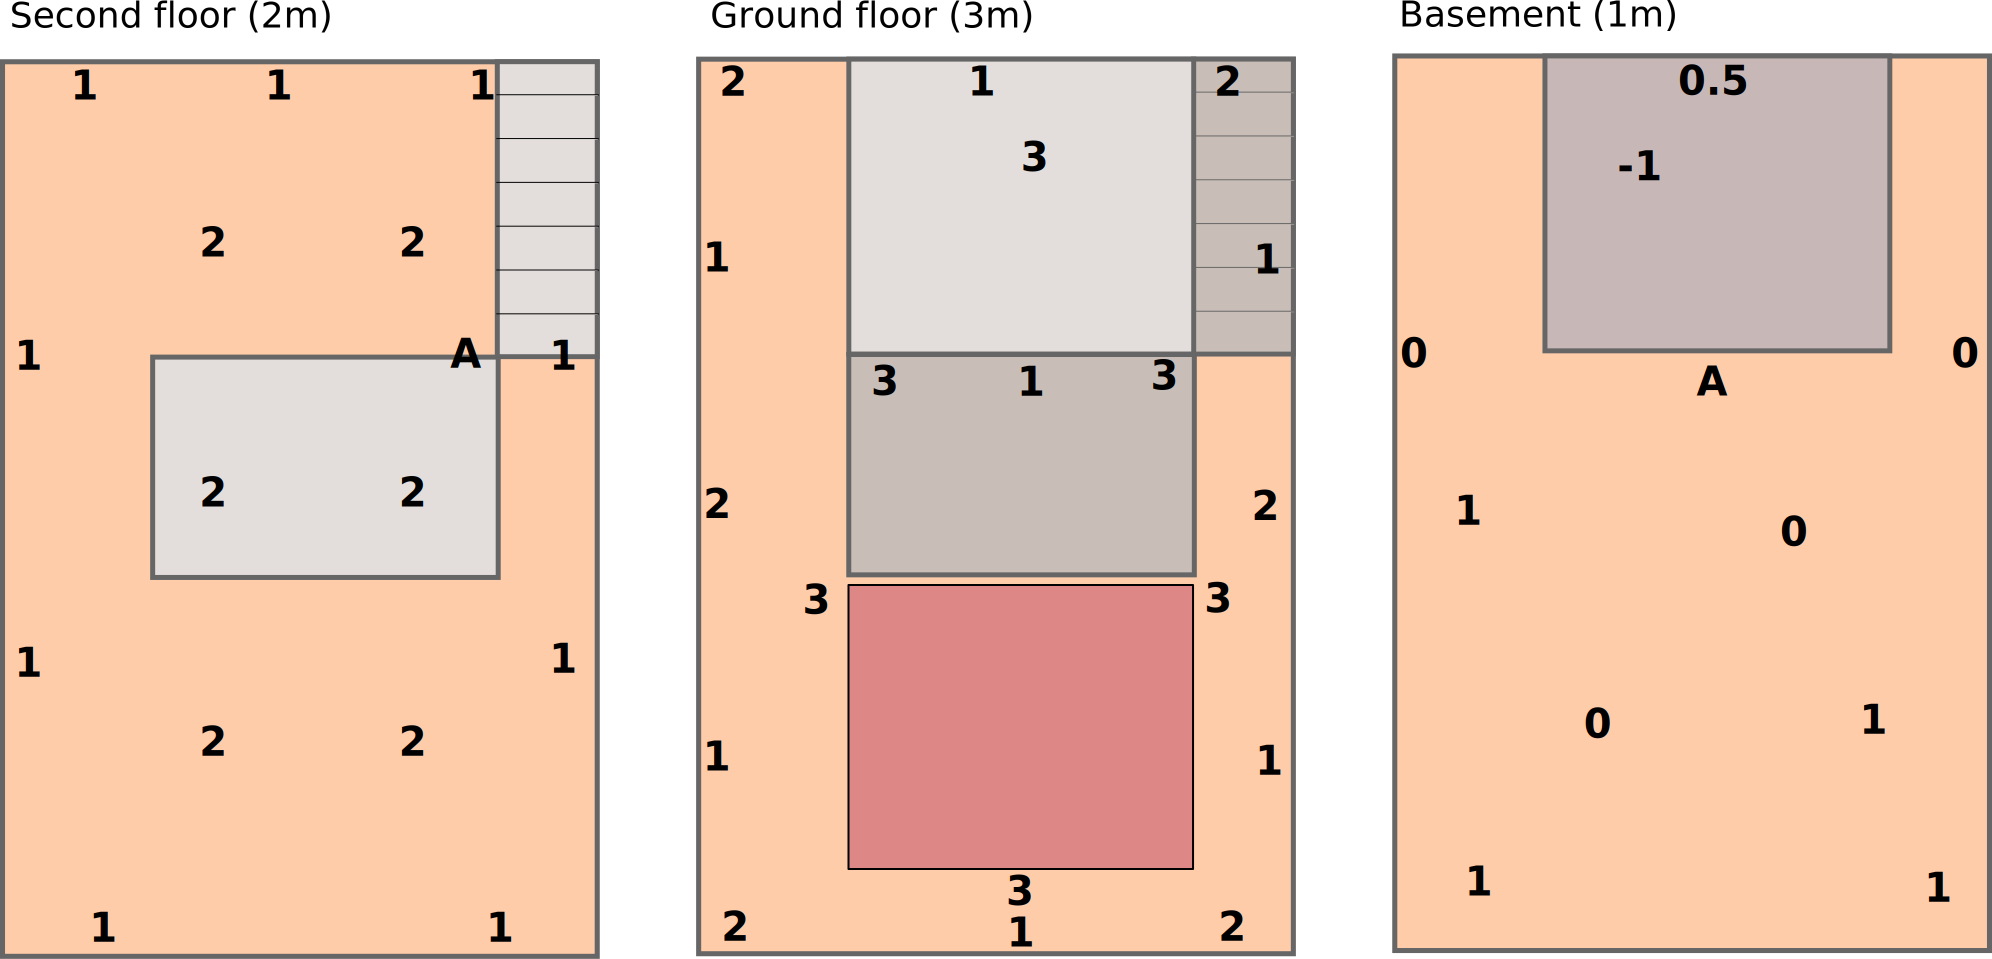
\includegraphics[width=\textwidth]{img/installPlan.pdf}
  \caption{Installation plan}
	\label{fig:install}
\end{figure}
\section{Maintenance}
\chapter{References}
%\renewcommand\refname{\vskip -1cm}
%\bibliographystyle{abbrv}
\bibliographystyle{plain}
\begingroup
\def\chapter*#1{}
\bibliography{bib}
\endgroup
%\bibliography{bib}
\nocite{*}

\end{document}
